\section{\proposed: On-device AI Agents Acceleration} 
\label{sect:proposed}

\subsection{\proposed Overview} \label{sect:proposed_overview}

\fig{fig:proposed_overview} provides an overview of our \proposed system. Building on the key observations in \sect{sect:motivation}, \proposed utilizes \prefill and \decode, which respectively accelerate the prefill and decode stages of agentic systems. The objective of these techniques is to speed up their target stages without compromising task accuracy or introducing substantial overhead in the resource-constrained on-device environment.

\textit{\prefill} (\sect{sect:proposed_prefill}) reconstructs the input prompt to minimize the amount of prompt that must be computed on the fly, effectively speeding up the prefill stage. \textit{\decode} (\sect{sect:proposed_decode}) accelerates the decode stage by using a simple lookup table as the draft model for speculative decoding. This lightweight draft model incurs no draft token generation overhead, while providing means to avoid the multi-token tax. With these two main components, \proposed accelerates the full system pipeline of on-device agents, targeting both the prefill (\prefill) and the decode (\decode) stages.


\begin{figure}[t!] \centering
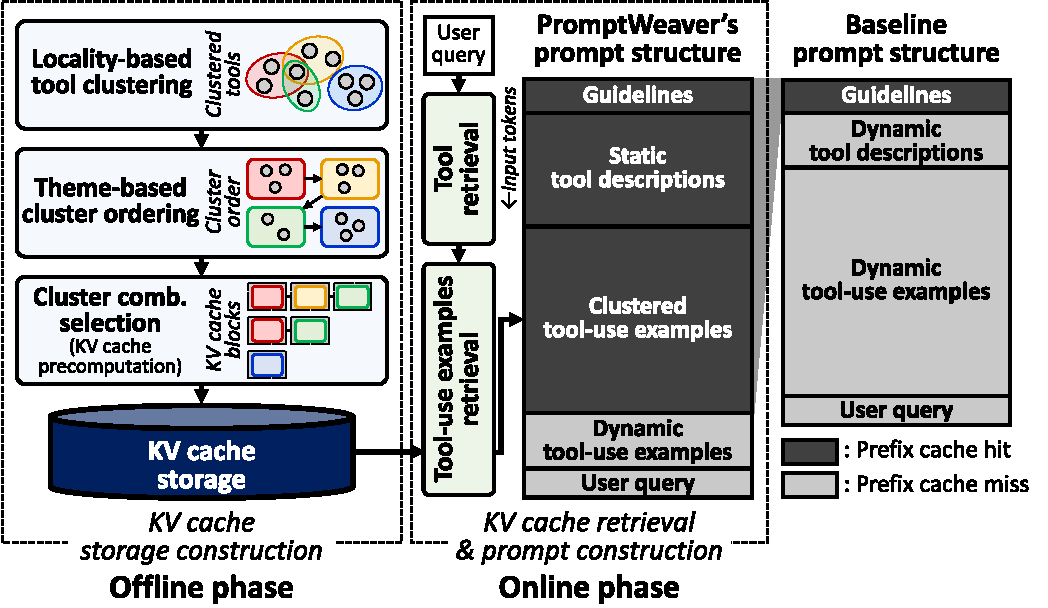
\includegraphics[width=\columnwidth]{./fig/proposed_prefill_overview}
\caption{
Overview of \prefill, divided into the offline (KV cache storage construction) and online phase (KV cache retrieval and prompt construction).
}
\Description{Overview of \prefill, divided into the offline (KV cache storage construction) and online phase (KV cache retrieval and prompt construction).}
\label{fig:proposed_prefill_overview}
\end{figure}


\begin{figure*}[t!] \centering
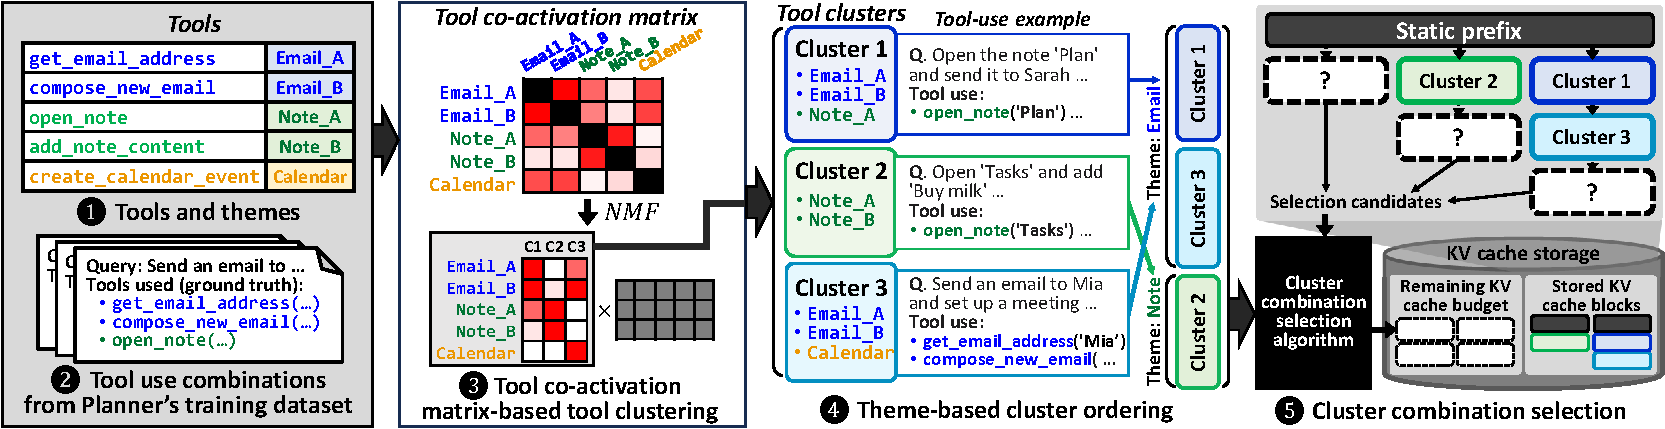
\includegraphics[width=1.0\textwidth]{./fig/proposed_prefill_detailed}
\caption{
\label{page:fig_edit_proposed_prefill_detailed}
Illustration of \prefill's offline KV cache precompute mechanism.
}
\Description{Illustration of \prefill's offline KV cache precompute mechanism.}
\label{fig:proposed_prefill_detailed}
\end{figure*}


\subsection{\prefill: Iso-accuracy Prompt Reconstruction} \label{sect:proposed_prefill}
\label{page:iso_accuracy}


In \sect{sect:prefill_analysis}, we identified three key traits of Planner inputs: (1) early dynamicity despite a large portion of static prompt, (2) tool co-activation locality, and (3) importance of single-tool examples in tool-use examples. \prefill exploits these observations to reduce uncacheable tokens while preserving accuracy. It rebuilds prompts so that most content forms a cacheable static prefix and the dynamic regions' KV caches can be reconstructed from KV caches stored inside the SSD. \fig{fig:proposed_prefill_overview} provides an overview of how \prefill introduces staticity without degrading accuracy. The reconstructed prompts consist of the following elements, in order: (1) all-inclusive static tool descriptions and guidelines, (2) clustered semi-cacheable tool-use examples, and (3) uncacheable dynamic tool-use examples.

{\bf Replacing early dynamic tokens.} The first dynamic fragment of prompt contains descriptions and usage guidelines for the selected tools. Because the set of tools selected depends on the input prompt and is thus determined at runtime, this section is where dynamicity is introduced. \prefill reconstructs this section to include descriptions and guidelines for \textit{all tools} available in the system. This replacement transforms the early dynamic segment into a larger but fully static prefix. Although this increases the size of the KV cache, it enables the prompts made static to be \emph{precomputed} and have their KV caches stored in the SSD. Since static prefixes can be cached once and reused across requests, our approach significantly reduces the number of uncacheable tokens in the prompt. Concretely, tokens previously marked as ``Static (uncacheable)'' in \fig{fig:agent_breakdown_token} are now part of the cacheable prefix, thereby reducing the dynamic token volume at runtime at the cost of a larger KV cache footprint.

In the process of inducing staticity, the input prompt grows longer. The average length of a single tool's description and guidelines is 120 tokens. For an agentic system using up to $t$ tools, including all descriptions and guidelines requires $120 \cdot t$ tokens. Even with a conservative estimate of 100 tools, our all-inclusive static tool description adds only 1.4 GB of additional KV cache stored on the SSD. In general, the performance benefits of our approach far outweigh the overhead introduced by this larger KV cache.


{\bf Tool-use example selection.} The remaining uncacheable input tokens primarily consist of tool-use examples. These examples are dynamic because they are selected at runtime based on the user prompt (\sect{sect:on_device_agents})~\cite{toolformer, rag_mcp, hugginggpt}. The all-inclusive static tool description and guidelines cannot be applied to tool-use examples for two reasons. First, supplying the Planner with all possible combinations of tool-use examples requires $2^t-1$ different combinations for a system with $t$ tools. For the current TinyAgent with 16 tools, this is equivalent to 800 GB of memory, increasing exponentially as more tools are supported ($memory \propto 2^t$). Second, the few-shot examples (i.e., tool-use examples) serve as templates and have a direct impact on the generation quality of LLMs. Adding such an excessive amount of tool-use examples would hamper the Planner's ability to extract relations between different tools~\cite{toolformer, rag_mcp, google_dev_function_calling}. Instead, \prefill chooses a fixed set of tool-use examples that can be reused across different queries at the offline phase through (1) co-activation locality-based tool clustering, (2) theme-based cluster ordering, and (3) cluster combination selection, as illustrated in \fig{fig:proposed_prefill_detailed}.



{\bf Co-activation locality-based tool clustering.}
In this stage, tools are clustered based on their co-activation locality (\fig{fig:tool_heatmap}). First, the tools are annotated with themes that relate to the tool's usage (\circlednum{1}), information that \prefill utilizes in the next theme-based cluster ordering stage. Then, \prefill refers to the Planner's training dataset (TinyAgent fine-tuning training dataset, \sect{sect:workload_characterization}) and iterates through all training data samples' ground truth labels to identify which tools are called together (\circlednum{2}). With this information, we generate a tool co-activation matrix, which is an adjacency matrix where each graph node corresponds to a tool and edges denote the number of times the corresponding pair of tools has been called together, and apply non-negative matrix factorization (NMF)~\cite{nmf} to cluster the tools based on the co-activation matrix (\circlednum{3}). This results in a total of eight clusters, each consisting of 2 to 6 tools. After the tools are clustered, we assign each cluster one tool-use example that uses exactly the tools in that cluster. These clusters then undergo theme‑based ordering and cluster combination selection (detailed later) before being stored in SSD for retrieval during inference. For example, when servicing a user query, ToolRAG retrieves the set of tools likely to be used for the request (\fig{fig:toolrag}(b)). A cluster is considered ``activated'' if it contains at least one of these tools, and the corresponding tool‑use examples from the activated clusters are included as few‑shot examples in the prompt (``Clustered tool‑use examples'' in \fig{fig:proposed_prefill_overview}).


{\bf Theme-based cluster ordering.}
To maximize KV cache reuse, clusters must be given a fixed ordering so that when the same combination of clusters are activated, the resulting KV cache yields the same value. That is, because having clusters A and B in order ``A-B'' and ``B-A'' yield different KV cache values, we impose a fixed ordering so that between clusters A and B, the order is always statically fixed as ``A-B'' (or ``B-A''). To maximize the amount of KV cache reuse under a fixed SSD capacity budget, \prefill applies theme-based clustering and cluster combination selection. The objective of theme‑based ordering is to place clusters that are frequently co‑activated adjacent to each other. Each cluster is assigned a theme based on which tool theme is most dominant in the cluster. Then, clusters with identical themes are grouped together and placed next to each other in a fixed order (\circlednum{4}). For example, clusters with the same theme ``Email'' are grouped together and placed adjacent to each other in order. If the tool \texttt{get\_email\_address} (\texttt{Email\_A}) is retrieved, clusters \texttt{1} and \texttt{3}, which include the tool, are activated. When the clusters are ordered based on their themes (after ordering in \circlednum{4}), having stored the KV cache of clusters ``\texttt{1}-\texttt{3}-\texttt{2}'' would fully cover for tool \texttt{get\_email\_address}, because if cluster \texttt{2} is not activated, we can cut out the mismatched tail (cluster \texttt{2}) and reuse the KV cache of ``\texttt{1}-\texttt{3}.'' However, if clusters were not grouped by themes and put in random order (before ordering in \circlednum{4}), it would require two cluster combinations (``\texttt{1}-\texttt{2}-\texttt{3}'' and ``\texttt{1}-\texttt{3}'') depending on whether or not cluster \texttt{2} is activated. Thus, with a fixed, theme-based ordering, \prefill can maximize prefix cache reuse across various requests.


\begingroup
\begin{algorithm}[t]
\caption{Cluster combination selection}
\label{algo:greedy_selection}
\begin{algorithmic}[1]
\footnotesize
  \STATE \textbf{Input:} KV cache budget $N$, Planner's training dataset $\mathcal{D}$
  \STATE \textbf{Output:} cluster combination KV cache $\mathcal{C}$
  \STATE Initialize $\mathcal{C} \gets \emptyset$
  \STATE Initialize prefixes $P \gets \{\text{all prefixes of sequences in }\mathcal{D}\}$
  \FOR{$i = 1$ to $N$}
    \STATE $\mathrm{options}\gets \emptyset$
    \FORALL{prefix $p$ in $P$}
      \IF{len($p$) == 1 or $p$[:-1] in $\mathcal{C}$}
        \STATE options.add($p$)
      \ENDIF
    \ENDFOR
    \STATE $\hat{p}=\displaystyle\argmax_{p \in \mathrm{options}} \left[ \mathrm{coverage}(\mathcal{D}, \mathcal{C}\cup\{p\}) {-} \mathrm{coverage}(\mathcal{D}, \mathcal{C}) \right]$
    \STATE $\mathcal{C}$.add($\hat{p}$)
  \ENDFOR
  \STATE \textbf{return} $\mathcal{C}$
\end{algorithmic}
\end{algorithm}
\endgroup


{\bf Cluster combination selection.}
The total number of possible cluster combinations is $2^C-1$ for $C$ ordered clusters. \prefill must carefully select combinations of clusters to store in the SSD to maximize KV cache reuse across requests, while keeping the SSD capacity overhead low. \algo{algo:greedy_selection} explains our proposed combination selection algorithm. Given a cache budget of $N$ clusters, starting from an empty KV cache set $\mathcal{C}$, all available cluster prefixes of all data samples in the Planner's training dataset ($\mathcal{D}$, same one used in locality-based clustering) are gathered (line 4). That is, if a sample activates clusters ``A-B-C'', its prefix sequences ``A,'' ``A-B,'' and ``A-B-C'' are all gathered. We define a new metric to give scores for each combination of cached clusters $\mathcal{C}$. For each activated cluster sequence in $\mathcal{D}$, the length of the longest cached prefix (i.e., how many leading clusters can reuse the KV caches in $\mathcal{C}$) is measured. The \textit{coverage} is defined by the sum of these per-sequence number of hit clusters in $\mathcal{D}$. A larger coverage implies a higher KV cache reuse across requests. Each step considers all candidate prefixes, either a singleton cluster (len($p$) == 1 in line 8, first dotted box in \circlednum{5}) or an extension to an existing sequence by one cluster of a prefix already owned ($p$[:-1] in $\mathcal{C}$ in line 8, second and third dotted boxes in \circlednum{5}), and computes how much coverage would increase if that candidate were added to the cached set (line 12). By greedily choosing the prefix that adds the largest amount of new coverage, the algorithm focuses on the most frequent early patterns without exploring every combination. The returned cluster combinations $\mathcal{C}$ have their KV cache precomputed and saved in the SSD for reuse at the online phase (\circlednum{5}). In \sect{sect:eval_prefill}, we show that with a cache budget size of just 15 clusters (5.87 GB of SSD capacity overhead), 74.4\% of tool-use examples are covered. This demonstrates that a small, carefully chosen subset of cluster combinations can serve the vast majority of prompt patterns, dramatically reducing SSD capacity overhead while preserving high KV cache reuse.

{\bf Preserving task accuracy with dynamic tool-use examples.} LLM output quality is known to be heavily dependent on the quality of few-shot examples in the prompt~\cite{gpt3, what_makes_good_examples, metalcl}. Therefore, composing the entirety of tool-use examples with clustered examples can have critical impact on the Planner accuracy. To alleviate this, we append single-tool examples\footnote{We add double-tool examples for a select few tools whose single-tool example was not present in the offline-generated database.} of activated tools, which we observed to be the most popular form of tool-use examples, to the end of the clustered examples. We also add top-$K$ ($0 \le K \le 4$) relevant examples from ToolRAG (\fig{fig:toolrag}(c)) to make up for any accuracy loss. In \sect{sect:eval_prefill}, our evaluations reveal that $K=1$ is the optimal choice in terms of accuracy, requiring only one additional tool-use example worth of dynamic tokens.


\subsection{\decode: Example-based Selective Speculative Decoding} \label{sect:proposed_decode}

\sect{sect:decode_analysis} uncovered two key properties of Planner and Arbiter output tokens: (1) decoded outputs are largely predictable from input prompts, and (2) applying speculative decoding na\"ively in on-device frameworks leads to suboptimal performance due to penalties from the multi-token tax and draft LLM latency overheads. We propose \decode to leverage this predictability without incurring these penalties. \fig{fig:proposed_decode_overview} illustrates the two main mechanisms of \decode: (1) lightweight draft token generation using an $n$-gram model~\cite{ngram} and (2) selective fallback to autoregressive generation when speculative decoding is likely to be inefficient.


\begin{figure}[t!] \centering
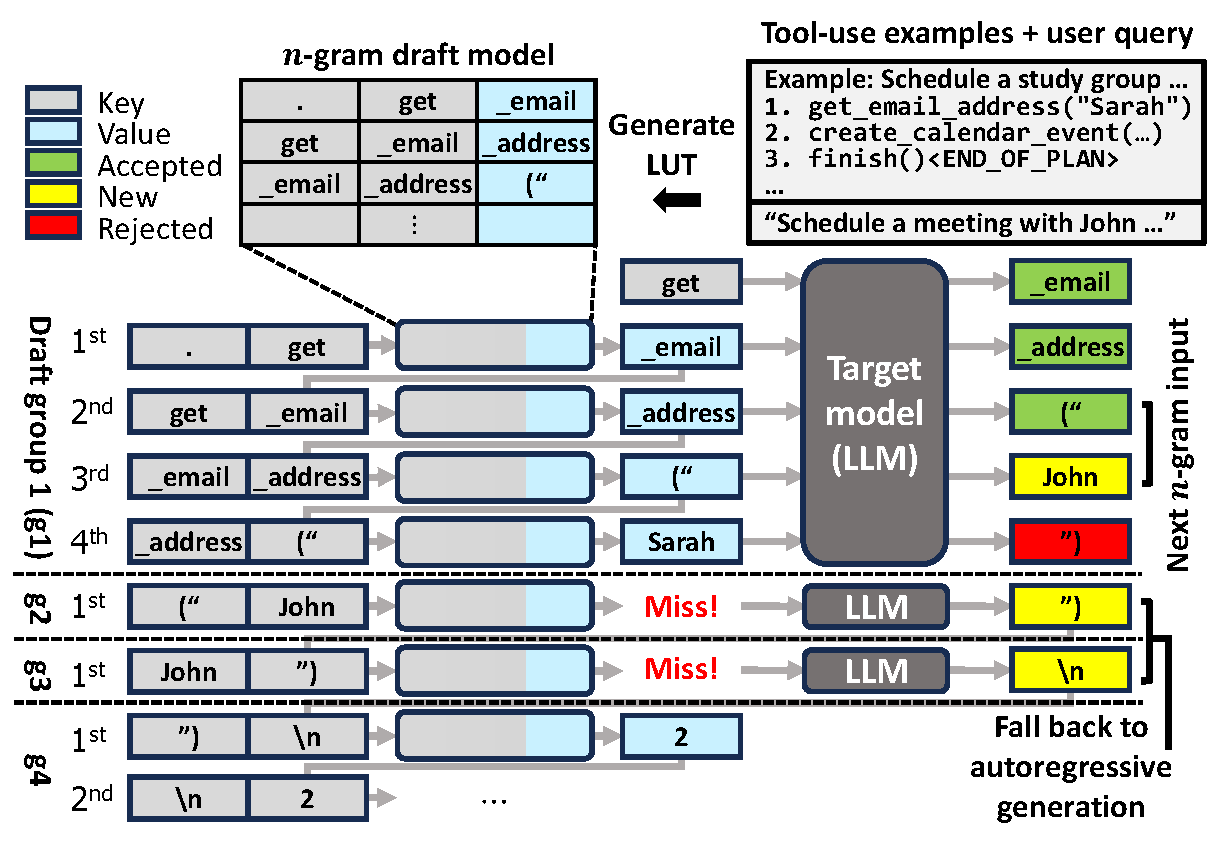
\includegraphics[width=\columnwidth]{./fig/proposed_decode_overview}
\caption{
Overview of \decode with trigram ($n{=}3$) LUT and draft token generation length of 4.
}
\Description{Overview of \decode with trigram ($n{=}3$) LUT and draft token generation length of 4.}
\label{fig:proposed_decode_overview}
\end{figure}


{\bf Draft LLM-free, example-based speculative decoding.}
A primary design objective of \decode is to remain lightweight while keeping decoded outputs tightly correlated with the input prompt. To this end, \decode builds a simple $n$‑gram lookup table (LUT) on the fly each time the agent receives a new user query. The LUT is populated as follows. To keep this table task-specific, we build the table from the few-shot examples (tool-use examples for Planner and decision examples for Arbiter) and the user query, all of which constitute a single stream of tokens. We then slide a window of $n$ consecutive tokens $t_{1:n}$ across this token stream, shifting one token at a time, and record each pair $\langle t_{1:n-1}, t_{n} \rangle$. The prefix $t_{1:n-1}$ serves as the key in the $n$‑gram LUT, and the corresponding value is the token $t_{n}$ that occurs most frequently with that key across all recorded pairs. Using this LUT, \decode generates each draft token by indexing the table with the most recent $n-1$ generated tokens (gray tokens in \fig{fig:proposed_decode_overview}) and the corresponding output becomes the draft token (blue token). A key advantage of \decode's LUT design is its minimal memory footprint, only amounting to a few KB. This lightweight design is ideal for on‑device AI systems, unlike conventional LLM‑based drafts, which consume hundreds of MB to several GB of memory (\tab{tab:draft_specdec_accuracy}).

Balancing $n$ is crucial for maximizing \decode's performance. With a small $n$, for example a unigram model ($n=1$), the LUT always proposes the single most frequent token from the few‑shot examples and user query, yielding low‑quality draft tokens. Conversely, a large $n$ provides richer context and higher‑quality drafts but often fails to predict unseen sequences, defaulting to random tokens when the $n-1$ prefix is not available in the LUT. We find that a trigram model ($n=3$) offers the best trade‑off between draft quality and LUT hit rate. The impact of $n$ is further explored in \sect{sect:eval_discussions}.


\begin{figure}[t!] \centering
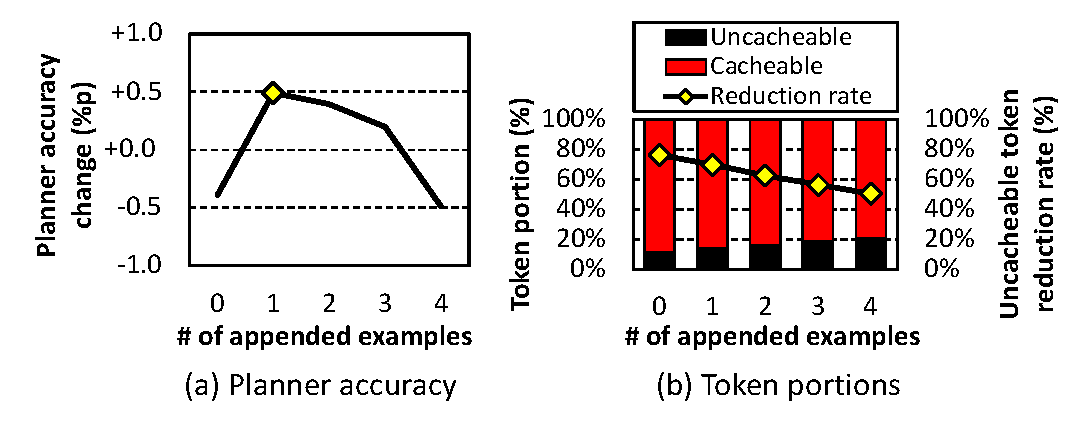
\includegraphics[width=\columnwidth]{./fig/eval_planner}
\caption{
\label{page:fig_clarification_eval_planner}
(a) Planner accuracy change vs. the number of appended tool-use examples.
(b) Share of cacheable and uncacheable tokens (left) and reduction in uncacheable tokens (right).
}
\Description{(a) Planner accuracy change vs. the number of appended tool-use examples.
(b) Share of cacheable and uncacheable tokens and reduction in uncacheable tokens.}
\label{fig:planner_accuracy_tokens}
\end{figure}


{\bf Multi‑token‑tax evasion with selective decoding.}
When the current $(n-1)$-token context is absent from the LUT, our $n$-gram draft model ``guesses'' a random token that rarely passes verification. Verification still generates the same output tokens via standard autoregressive decoding and incurs the multi‑token tax, ultimately slowing down overall token generation. \decode mitigates this limitation by opting out of speculative decoding when no speedup is expected. Specifically, \decode consults the LUT before generating the first draft token: if no valid entry exists, it immediately falls back to standard autoregressive decoding (yellow tokens in \fig{fig:proposed_decode_overview}). This safeguard ensures speculative decoding is used only when its speedup outweighs the verification cost. Because the $n$‑gram LUT deterministically knows which contexts it covers, this decision incurs zero overhead—an assurance LLM‑based drafts cannot provide. Once the first draft token is retrieved from the LUT, the remaining tokens in that group are generated regardless of subsequent misses.